\chapter{\label{detchar}Detector Characterisation with SOAP}
%%%%%%%%%%%%

When searching for \ac{GW} signals, it is important to understand the origins of noise in the the detectors data which does not originate from an astrophysical source.
A large fraction of \ac{GW} search algorithms, including SOAP above, assume that the detectors noise follows a Gaussian distribution.
However, the detectors contain artefacts which are not distributed as a Gaussian. 
These artefacts can negatively affect many searches for \ac{GW} as they can be easily mistaken for a real \ac{GW} signal.
Some of the potential sources of these artefacts have been mentioned in Sec.~\ref{intro:detector:noise}. 
There are many different classes of artefact such as: glitches, \joe{fill}, instrumental lines and .
To conduct a reliable search there are two main tasks which are necessary for detector characterisation.
The first is identifying the artefact such that any search knows that part of data is contaminated.
The search can then remove that section of data, or use more sophisticated techniques to deal with the artefact \citep{}.
The second task is to find the source of the artefact. 
If the source of the artefact is found, it can potentially be removed or limited for future data runs.
The majority of this section will focus on a particular class of artefact called instrumental lines and how the affect \ac{CW} searches.





%%%%%%%%%
%%%%%%%%%%
\section{Instrumental lines}
%%%%%%%%%
%%%%%%%%%

Instrumental lines have the general structure that they are persistent noise artefacts.
There are many classes of instrumental line including: narrow, fixed frequency spectral artefacts or broad features which wander in frequency.
A few examples of these are shown in Fig.~\ref{}. 

\begin{figure}
    \centering
    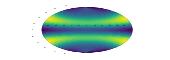
\includegraphics[width=\textwidth]{testimg.png}
    \caption{Caption}
    \label{fig:my_label}
\end{figure}

As described in Sec.~\ref{searchcw}, \ac{CW} are long duration signals with a slowly varying frequency.
In the case of an isolated neutron star, the signal which is searched for is narrow-band and a fixed frequency which is Doppler modulated by the earths rotation and orbit.
For certain areas of parameter space, the astrophysical signal of an isolated neutron star can appear very similar to an instrumental line. 
Many of these lines can be ignored if they appear in a single detector, or a statistic such as in Sec.~\ref{viterbi:las} can be used to limit their effect.
However, there are many examples of instrumental line which appear at the same or similar frequencies in multiple detectors.
These pose a real challenge to some \ac{CW} searches, and require a lot of investigation to limit their affect.


The origin of many instrumental lines have been identified.
Many of these can and have been removed, however, some cannot be removed. 
An example of a line which cannot be removed is the violin modes of the suspensions of the detectors mirrors. 
These areas of the frequency spectrum are generally assumed to be contaminated and are ignored in any search.




\begin{itemize}
    \item instumental lines are long or short duration detector artifacts
    \item can be narrow and short or broad and long duration
    \item many examples from known sources
    \item many searches currently exist which look through data
    \item . wandering lines are a large problem as hard to track especially when weak
\end{itemize}

%%%%%%%%%%
%%%%%%%%%%
\section{Identifying and monitoring instrumental lines}
%%%%%%%%%%
%%%%%%%%%%

When a detector is running, it is very important to identify instrumental lines and monitor them.
This can then lead to either locating the origin of the line such that it can be removed, or allowing it to be flagged for other search algorithms.
The lines are generally identified in the \ac{GW} channel, this is the output of the detector which \ac{GW} are observed and is the data using is previous chapters.

As well and the \ac{GW} channel the detector records many different channels known as auxillary channels. 
These channels monitor many components of the detector and anything which may affect the \ac{GW} channel.
For example, the seismomenter which are located near the corner stations and end stations are all channels which are monitered. 

Some of the channels which are useful for monitoring and locating lines include: \ac{PEM} , .......
\ac{PEM} channels include instrumental such as magnetometers and ........
These are useful to investigate alongside the main \ac{GW} channel.
The main goal is to reduce the number of artefacts in the \ac{GW} such that it is as close to Gaussian noise as possible.
If an artefact shows up in the \ac{GW} channel in coincidence with one of the \ac{PEM} or other channels, then this is an indicator that the artefact originates from something related to that \ac{PEM}.
For example, 


%%%%%%%%%%%
%%%%%%%%%%%
\section{Identifying and cleaning lines with SOAP}
%%%%%%%%%%%
%%%%%%%%%%%%

\begin{itemize}
    \item overview of soap search and what type is used for line searches
    \item how this is applied and how to interpret the output for lines searches
    \item SOAP can identify weak lines when they are wandering or fixed frequency
    \item 
\end{itemize}


%%%%%%%%%%%
%%%%%%%%%%%%
\section{Summary pages}
%%%%%%%%%%%
%%%%%%%%%%%%%

\begin{itemize}
    \item why summary pages are useful 
    \item how to read them and what they mean
    \item how to use the information with other searches
\end{itemize}
